\chapter{Boh}

\section{Introduzione}

In questa parte di corso siamo interessati a definire le classi di complessita'. Ci sono alcune
differenze con la complessita' intesa in senso algoritmo.

Come si valuta la complessita' computazionale (il costo di far funzionare dei programmi)?
Tipicamente si misura il costo in funzione del consumo di una determinata risorsa. Abbiamo
fondamentalmente due risorse principali di riferimento nella computazione: tempo e spazio.

Perche' non usiamo altre risorse? Ad esempio il consumo di energia elettrica? La temperatura della
CPU? Potremmo. Cio' pone una questione interessante: che relazione c'e' tra queste risorse? Ad
esempio, sapendo quanto tempo richiede un programma per essere eseguito sappiamo qualcosa
sull'occupazione di memoria? Il viceversa e' un po' piu' delicato.

Come misuriamo il costo computazionale? Tipicamente si e' interessati al comportamento asintotico di
un programma, al crescere della dimensione degli input. Potrei avere un'analisi puntuale, e si puo'
fare. Di solito e' il punto di partenza dell'analisi del costo. Si puo' pero' fare una
considerazione diversa e chiedersi quanto scala il programma al crescere della dimensione dei dati
di input.

Si possono ovviamente avere delle fluttuazioni nei dati e quindi nel comportamento del programma.
Noi consideriamo di solito il caso pessimo. Questo e' utile perche' mi da' un limite al peggio che
puo' succedere. Potrebbe a volte essere interessante fare un'analisi del caso medio, che pero' e' in
genere molto piu' complessa della corrispettiva per il caso pessimo (bisogna conoscere la
distribuzione dei dati di input ad esempio).

Puo' succedere che un programma possa avere un comportamento ``pesante'' all'inizio e leggero al
crescere dell'input. La nostra analisi ignora il primo aspetto.

Un'altra parte importante riguarda il meccanismo di calcolo.

Ci chiediamo anche quanto la misura del tempo e dello spazio dipenda dal particolare modello
computazionale che usiamo.

Noi faremo analisi e prescidere dalle costanti. $1000*n^{2}$ e $10*n^{2}$ sono equivalenti per noi.
E' un tentativo di dissociarsi dal particolare modello di calcolo usato. Ma funziona? O la nostra
misura di complessita' rimane vincolata ad un particolare modello di calcolo. Ad esempio, abbiamo
programmi con complessita' diverse a seconda dell'architettura ($n^{2}$ vs $n^{6}$ per esempio)?.
Non e' nemmeno scontato che il processo di compilazione mantenga la complessita' del programma in
codice sorgente (ad esempio per considerazioni legate all'implementazione del linguaggio). Noi
faremo riferimento a macchine teoriche (Macchine di Turing). Ci chiederemo: data una macchina con
$n$ nastri riusciamo a calcolare uno stesso algoritmo con la stessa complessita' che avremmo con una
macchina con 1 nastro? La risposta sara' no. Questa e' una forte differenza rispetto alla teoria
della complessita' (il numero di nastri non ha alcuna influenza sulla calcolabilita' di una
funzione).

Consideremo quanto sia significativo dire che un certo problema ha una data complessita'.

Tra i modelli che considereremo ci sara' quello non deterministico, che e' un po' strano. Dovremo
capire perche' siamo interessati a questa nozione. Il motivo principale e' che ci interessa la
classe $\NPClass$, che contiene tanti problemi con una complessita' computazionale elevata con gli algoritmi
odierni e con delle buone euristiche. Non si e' ancora dimostrato che non esista un modo di
risolvere questi problemi in tempo polinomiale con una macchina deterministica. Cercheremo di capire
perche' e' cosi' complicato da dimostrare.

Perche' $\NPClass$ e' cosi' interessante? Perche' e' la classe di problemi per i quali non sappiamo se
abbiamo degli algoritmi efficienti per risolverli ma per i quali abbiamo metodi di verifica di una
soluzione efficienti. Non e' scontato che esista un modo di verificare una soluzione in maniera
efficiente per un dato problema.

Prendiamo ad esempio il problema della soddisfacibilita' proposizionale. Come tanti dei problemi che
vedremo e' un problema decisionale (risposta si'/no). Il nostro programma deve dirmi si' se una data
formula e' soddisfacibile e no altrimenti. E' possibile avere un certificato che ``giustifichi'' la
risposta. Per SAT questo certificato puo' essere l'assegnazione di valori alle variabili che
soddisfa la proposizione. In tempo lineare posso fare la sostituzione e verificare se la formula
ottenuta e' valida.

Il problema della tautologicita' non e' di questa categoria. Si puo' dare un certificato compatto
per questo problema? Si direbbe di no, ma non si e' ancora dimostrato il contrario.

Il certificato per essere compatto deve avere dimensione polinomiale.

Che un problema sia in $\NPClass$ e' utile da sapere per decidere come verificare in maniera efficiente che
una soluzione sia valida.

I problemi in $\NPClass$ sono spesso detti intrattabili. Questo forse e' esagerato. Questi problemi
sono comuni, si usano tante euristiche e tecniche per ottenere delle soluzioni parziali che vanno
gia' abbastanza bene. C'e' molto di peggio. Perfino in $\PClass$ ci sono problemi ``intrattabili'',
ad esempio con complessita' superiore al $n^{3}$, molto peggiori dei piu' famosi problemi in
$\NPClass$.

In questa parte del corso siamo interessati a cosa siamo in grado di calcolare in tempi ragionevoli.
La calcolabilita' in senso astratto non rende, da sola, un problema pratico.

Purtroppo in complessita' siamo dipendenti dal modello di calcolo (nella definizione del costo). E'
importante capire quanto dipendiamo.

Siamo interessati a trasformazioni che ci portino da un modello di calcolo ad un altro. Siamo
interessati anche a capire quanto ci costa simulare, in modo deterministico, modelli di calcolo non
deterministici.

Ci sono inclusioni che sono congetturate che tuttavia non sono facili da dimostrare. La piu' famosa
e' la relazione tra $\PClass$ e $\NPClass$. Pare che manchi ancora la tecnica matematica corretta
per affrontare queste problematiche, la scienza e' ancora incompleta.

Noi misuriamo la complessita' computazionale in funzione della dimensione dei dati di input. Questo
perche' di solito accettiamo stringhe di bit che rappresentano l'input in modo compatto. Con un
alfabeto almeno binario abbiamo almeno una rappresentazione logaritmica dei dati in input. Ovvero,
la rappresentazione di un numero $n$ ha lunghezza che e' di ordine $\log(n)$.

Tutte le volte che abbiamo algoritmi che lavorano con numeri la dimensione dell'input e'
logaritmica. Se l'input e' $n$ e la complessita' e' lineare in $n$ la complessita' dell'algoritmo
non e' lineare, bensi' esponenziale nella dimensione dell'input.

Qui c'e' una leggera differenza tra la teoria della complessita' e la teoria algoritmica della
complessita'. In algoritmica le operazioni artimetiche vengono considerate avere costo costante.
Cio' non e' necessariamente sbagliato, dato che si considerano interi con una dimensione massima
(limitata dalla grandezza della parola di memoria). Fintanto che ho un bound alla dimensione dei
dati tutte le operazioni hanno costo costante. Se facessimo operazioni su interi di grandezza
arbitraria queste assunzioni non varrebbero piu', e il costo dipende dall'implementazione usata, e
sicuramente non sara' costante.

Noi siamo interessati a complessita' asintotiche, non possiamo assumere che i nostri interi abbiano
dimensione fissata. Per noi possono avere dimensione arbitraria.

Rispetto alle funzioni $f:\Nat \to \Nat$, che utilizziamo per misurare il costo di un'operazoine,
possiamo fare una suddivisione in classi, dette \textbf{notazioni d'ordine}.

Le notazioni d'ordine sono insiemi di funzioni. La classe piu' importante, a cui faremo riferimento,
e' la $O(f)$.

\begin{defn}
    Sia $f: \Nat \to \Nat$. Definiamo le seguenti notazioni d'ordine:
    \begin{enumerate}
        \item $O(f) = \set{g:\Nat \to \Nat \mid \exists c \forall n, g(n) \leq c f(n) + c}$; e' la
        classe delle funzioni che crescono al piu' come $f$;
        \item $o(f) = \set{g:\Nat \to \Nat \mid \forall c \exists n_{0} \forall n \geq n_{0}, c g(n)
        + c \leq f(n)}$; e' la classe delle funzioni che crescono meno rapidamente di $f$;
        \item $\Omega(f) = \set{g:\Nat \to \Nat \mid f \in O(g)}$; e' la classe delle funzioni che
        crescono almeno quanto $f$;
        \item $\Theta(f) = O(f) \cap \Omega(f)$; e' la classe delle funzioni che crescono come $f$;
    \end{enumerate}
\end{defn}

Abbiamo che valgono le seguenti proposizioni:
\begin{itemize}
    \item $\forall c > 0, O(cf) = O(f)$ 
    \item se $f_{1} \in O(g_{1})$ e $f_{2} \in O(g_{2})$ allora $f_{1} + f_{2} = O(g_{1} + g_{2})$
    \item se $f_{1} \in O(g_{1})$ e $f_{2} \in O(g_{2})$ allora $f_{1}\cdot f_{2} = O(g_{1} \cdot g_{2})$
\end{itemize}

La definizione d'ordine e' indipendente dalle costanti. Questo e' importante perche' vogliamo
renderci indipendenti dalle unita' di misura. Se cambia l'unita' di misura non vogliamo che cambi
anche l'ordine di complessita'. E' analogo al rendersi indipendenti dalle prestazioni del processore
rispetto alla complessita'.

Sia $g(n) > 0$ per ogni $n$. Valgono le seguenti proposizioni:
\begin{itemize}
    \item se $\lim_{n \to \infty}\frac{f(n)}{g(n)} = l \not= 0$, allora $f \in O(g)$ e $g \in
    O(f)$
    \item se $\lim_{n \to \infty}\frac{f(n)}{g(n)} = 0$ o $\lim_{n \to \infty}\frac{g(n)}{f(n)} =
    \infty$, allora $f \in O(g)$ e $g \notin O(f)$
    \item $\lim_{n \to \infty}\frac{f(n)}{g(n)} = 0$ se e solo se $f \in o(g)$
\end{itemize}

$f \in o(g)$ implica $f \in O(g)$ ma non il viceversa.

Scrivere $g \in O(f)$ e' equivalente a scrivfere $O(g) \subseteq O(f)$.

Se il limite all'infinito del rapporto tra $f$ e $g$ e' uguale ad una costante diversa da 0 abbiamo che
$f$ e $g$ hanno lo stesso comportamento asintotico.

Quando cerchiamo l'ordine di grandezza cerchiamo la funzione piu' semplice che mi indichi il
comportamento asintotico della mia funzione. Un polinomio di quarto grado e' sicuramente $O(n^{5})$,
ma l'ordine piu' semplice che useremmo e' $O(n^{4})$.

Abbiamo che:
\begin{itemize}
    \item per ogni costante $c$, $n^{c} \in O(c^{n})$, ma $c^{n} \notin O(n^{c})$: l'esponenziale
    cresce piu' velocemente di qualsiasi polinomio;
    \item per ogni $a,b$, $\log_{a}(n) \in O(\log_{b}(n))$;
    \item per ogni $a,b$, se $a < b$, $b^{n} \notin O(a^{n})$;
    \item $O(n \log(n)) = O(\log(n!))$ e $O(n^{n}) = O(n!)$ 
\end{itemize}

Per le complessita' logaritmiche la base e' ininfluente. Per le complessita' esponenziali invece la
base e' influente.

Le ultime uguaglianze sono vere in luce delle disuguaglianze di Stirling:
\begin{equation*}
    e\left(\frac{n}{e}\right)^{n} \leq n! \leq e n \left(\frac{n}{e}\right)^{n}
\end{equation*}

Nella tabella \ref{algocomp} e' possibile osservare le complessita' di alcuni algoritmi noti:
\begin{table}[h]
    \begin{tabular}{|l|l|p{7cm}|}
        \hline
        \textbf{Ordine} & \textbf{Nome} & \textbf{Esempio} \\
        \hline
        $O(1)$ & costante & operazioni su strutture dati finite \\
        \hline
        $O(\log n)$ & logaritmico & ricerca di un elemento in un array ordinato o in un albero
        bilanciato \\
        \hline
        $O(n)$ & lineare & ricerca di un elemento in array disordinati/liste; somma di due interi con la
        tecnica del riporto\\
        \hline
        $O(n\log n)$ & quasi-lineare & Fast Fourier transform; merge-sort, quicksort (caso medio)\\
        \hline
        $O(n^{2})$ & quadratico & prodotto di due interi; bubble sort e insertion sort \\
        \hline
        $O(n^{c})$, per $c > 1$ & polinomiale & parsing di grammatiche contestuali; simplesso (caso
        medio)\\
        \hline
        $O(c^{n})$, per $c > 1$ & esponenziale & soluzione del problema del commesso viaggiatore con
        tecniche di programmazione dinamica; costruire la tabella di verita' di una proposizione \\
        \hline
        $O(n!)$ & fattoriale & soluzione del problema del commesso viaggiatore mediante ricerca esaustiva \\
        \hline
    \end{tabular}
    \caption{Complessita' di alcuni algoritmi noti}
    \label{algocomp}
\end{table}

La tabella \ref{algocomp} considera complessita' in tempo.

Ha senso di parlare di complessita' in tempo sublineari? Si potrebbe rispondere naturalmente di si',
portando due esempi famosi (binary search e alberi bilanciati). Questo pero' ha senso se suppongo
che la struttura che sto usando e' gia' data e non devo rileggerla ogni volta. Se dovessi leggere
ogni volta una struttura dati di grandezza $n$ allora la complessita' sara' quantomeno lineare nella
dimensione dell'input, poiche' l'input va letto.

Si suppone spesso che le complessita' in tempo sublineari non abbiano molto senso. Lo acquistano
solo se facciamo significative assunzioni sul problema in questione.

Molti problemi con algoritmi di complessita' esponenziale nel caso pessimo fanno anche parte di
$\NPClass$. Quantomeno ci e' agevole verificare che una soluzione sia valida.

Il grafo e' una struttura dati molto ricca in informatica. Ha inoltre una definizione matematica
molto precisa.

\begin{defn}
    Un grafo finito e' una coppia $(V,E)$:
    \begin{enumerate}
        \item $V$ e' un insieme finito di vertici;
        \item $E \subseteq V \times V$ e' una relazione che definisce l'insieme degli archi.
    \end{enumerate}
\end{defn}

Un grafo $G = (V,E)$ e' \textbf{non orientato} quando la relazione $E$ e' simmetrica e non
riflessiva.

Noi considereremo sempre grafi finiti ($V$ e $E$ finiti).

\begin{defn}
    Sia $G = (V,E)$ un grafo.
    \begin{itemize}
        \item due vertici $u,v \in V$ sono adiacenti se esiste un arco $(u,v) \in E$;
        \item un cammino e' una sequenza di coppie di vertici dove per ciascuna coppia consecutiva
        i due vertici sono adiacenti;
        \item un cammino e' semplice se tutti i vertici sono distinti;
        \item un ciclo e' un cammino dove il primo e l'ultimo vertice coincidono e dove non ci sono
        ulteriori ripetizioni di vertici
    \end{itemize}
\end{defn}

\begin{defn}
    Sia $G = (V,E)$ un grafo.
    \begin{itemize}
        \item Un cammino (ciclo) Hamiltoniano in $G$ e' un cammingo (ciclo) che comprende ciascun
        vertice del grafo una sola volta;
        \item Un ricoprimento di vertici per $G$ e' un sottoinsieme $V_{0} \subseteq V$ tale che
        ogni arco $e \in E$ ha almeno un'estremita' in $V$;
        \item $G$ e' $n$-colorabile se esiste una funzione di colorazione $\col: V \to
        c_{1},\dotsc,c_{n}$ tale che vertici adiacenti hanno colori diversi, ovvero
        \begin{equation*}
            (u,v) \in E \implies \col(u) \not= \col(v)
        \end{equation*}
        \item $G$ e' completo se ogni coppia di nodi distinti e' connessa da un arco
        \item Una cricca di $G$ e' un suo sottografo completo $G' = (V',E')$, ovvero tale che $V'
        \subseteq V$ e $E' = V' \times V' \subseteq E$
        \item Un insieme indipendente in $G$ e' un sottoinsieme di vertici $V' \subseteq V$ tale che
        per ogni coppia di vertici $u,v \in V' \implies (u,v) \notin E$.
    \end{itemize}
\end{defn}

Un grafo $G=(V,E)$ ammette sempre dei ricoprimenti ($V$ stesso ad esempio). Inoltre se $R$ e' un
ricoprimento di $G$ ogni suo sovrainsieme lo e'. Quello a cui siamo interessati e' un ricoprimento
minimo di solito. Non e' detto che un ricoprimento di una certa dimensione sia unico.

Un grafo ammette sempre anche degli insiemi indipendenti (ad esempio l'insieme vuoto o il singoletto
$\set{v}$, se $v \in V$). Inoltre se $I$ e' un insieme indipendente di $G$ ogni suo sottoinsieme lo
e'. Siamo interessati a insiemi indipendenti significativi, ovvero massimi.

Il complementare di un ricoprimento e' sempre un insieme dipendente, e viceversa. In particolare il
complementare di un ricoprimento minimo e' un insieme indipendente massimo. Cercare uno e'
equivalente a cercare l'altro.

Ogni grafo ammette delle cricche (ad esempio la cricca di dimensione 1 o 2). Inoltre se $C$ e' una
cricca di $G$ allora ogni suo sottoinsieme lo e'. Siamo ancora una volta interessati a cricche di
dimensione massima.

Questi sono tutti problemi interessati e tipicamente $\NPClass$ completi.

Il problema della colorabilita' cambia complessita' in base al valore di $n$. Ad esempio, la
2-colorabilita' e un problema in $\PClass$, la 3-colorabilita' e un problema $\NPClass$ completo. E'
una tecnica comune quella di restringere un problema per diminuire la complessita'. A volte si
riesce a ridursi ad un problema che ha algoritmi polinomiali (per casi particolari).

C'e' un legame tra l'esistenza di un algoritmo di verifica polinomiale per la soluzione ad un
problema e l'appartenenza alla classe $\NPClass$.

E' importante fare delle considerazioni sulla rappresentazione che facciamo dei grafi. Questa
infatti influenza l'analisi della complessita' che andremo a fare.

Si rappresenta solitamente un grafo mediante matrice di adiacenza.

\begin{defn}
    La matrice di adiacenza $M_{G}$ di un grafo $G = (V,E)$ e' la matrice definita nel modo
    seguente:
    \begin{equation*}
        M_{G}(u,v) = 1 \iff (u,v) \in E
    \end{equation*}
\end{defn}

Se non ho ipotesi sul numero di archi in un grafo posso supporre che il grafo abbia $O(n^{2})$ archi.
In questo caso la rappresentazione con matrice e' conveniente.

Se il grafo e' sparso sono piu' convenienti altre rappresentazioni.

La complessita' di solito e' data in funzione di $V$ e di $E$.

Un algoritmo molto importante sui grafi e' quello della raggiungibilita', ovvero determinare se
esiste un cammino tra due nodi del grafo. Si puo' fare mediante una visita.

Una visita in generale si svolge nel seguente modo:
\begin{enumerate}
    \item si partiziona il grafo in tre parti:
    \begin{enumerate}
        \item nodi gia' processati (nodi Done)
        \item frontiera corrente (nodi Current)
        \item nodi ancora da visitare (nodi Todo)
    \end{enumerate}
    \item\label{visitLoop} si prende un nodo da cardine e lo si processa (nel caso della raggiungibilita' vediamo se
    siamo arrivati in fondo).
    \item fatto cio', vediamo che nodi posso raggiungere dal nodo cardine
    \begin{enumerate}
        \item se il nodo e' done lo ignoro
        \item se il nodo e' todo estendo Current con il nodo
    \end{enumerate}
    \item estendo Done con il nodo cardine
    \item si riparte da \ref{visitLoop} fino a che l'insieme Current non risulti vuoto
\end{enumerate}

Una rappresentazione grafica del processo e' data dalla figura \ref{GraphVisit}.

\begin{figure}[h]
    \begin{center}
        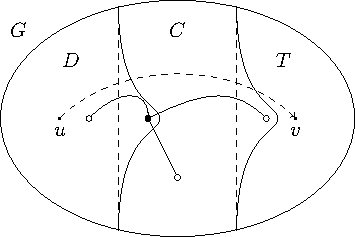
\includegraphics{img/GraphVisit.pdf}
    \end{center}
    \caption{Rappresentazione grafica dello schema di algoritmo di visita}
    \label{GraphVisit}
\end{figure}

La complessita' e' lineare nel numero degli archi. Tutti gli archi devono essere visitati almeno una
volta, se voglio fare una visita completa.

Tanti algoritmi di visita possono essere visti come modifiche di questo algoritmo qui andando a
lavorare su come gestisco l'aggiunta di nuovi nodi che vedo a current. Se aggiungo in cima ho una
politica in profondita' (LIFO). Nel caso duale avrei una visita in larghezza. Queste sono
fondamentalmente le uniche due visite che hanno senso.

Visita in profondita' e larghezza hanno caratteristiche diverse. La visita in profondita' non
garantisce di trovare il cammino di lunghezza minima, quella in larghezza permette di trovare sempre
il cammino di lunghezza minima che connette i miei due nodi. La ricerca di un cammino minimo tra due
nodi e' un'operazione semplice.

E' semplice calcolare il cammino piu' lungo in un grafo? Se lo fosse potrei controllare la sua
lunghezza. Se questa e' uguale a $n$ allora abbiamo anche un cammino hamiltoniano. La ricerca di un
cammino lungo e' equivalente alla ricerca di un cammino hamiltoniano. E quindi e' anche un problema
in $\NPClass$ (lo vedremo piu' avanti).

In un certo senso il duale di un problema semplice e' un problema difficile (cammino minimo vs.
cammino massimo). Non basta una semplice scansione dei cammini per trovare il piu' lungo, ma devo
considerarli tutti. Questo rende piu' complessa la ricerca.
